\section{Технологическая часть}
    \par В данном разделе обосновывается выбор средств программной реализации. 
    Описываются основные особенности реализации. 
    Приводятся примеры работы программно-алгоритмического комплекса.

    \subsection{Выбор средств реализации программно-алгоритмического комплекса}
    \subsubsection{Выбор языка программирования}
        \par В качестве языка программирования для реализации программного комплекса был выбран Swift. 
        Выбор языка обусловлен следующими причинами:
        \begin{itemize}
            \item[---] программный интерфейс AudioToolbox написан на языке программирования Swift;
            \item[---] наличие механизма подсчёта ссылок ARC, который автоматически деалоцирует неиспользуемые объекты памяти;   
            \item[---] наличие достаточного опыта программирования на данном языке, что позволит сократить время разработки программного комплекса;
        \end{itemize}

    \subsubsection{Выбор среды разработки}
        \par В качестве среды разработки была выбрана интегрированная среда разработки Xсode \cite{xcode} по следующим причинам:
        \begin{itemize}
            \item[---] поддержка компиляции программного обеспечения для симуляторов мобильных устройств на операционной системе iOS 
            для тестирования разрабатываемого программного комплекса;
            \item[---] наличие отладчика, поддерживающего многопоточную работу алгоритмов;   
            \item[---] наличие анализатора состояния ЦПУ, ОЗУ, сетевой нагрузки мобильных устройств и симуляторов на операционной системе iOS;
            \item[---] наличие механизма кэширования объектных файлов, который сокращает повторную компиляцию программного обеспечения;
            \item[---] наличие встроенной системы сборки программного обеспечения; 
        \end{itemize}

    \subsection{Диаграмма классов реализуемого программно-алгоритмического комплекса}
        \par На рис. \ref{fig:uml} представлена диаграмма классов реализуемого программного комплекса.
        \begin{figure}[!h]
            \center{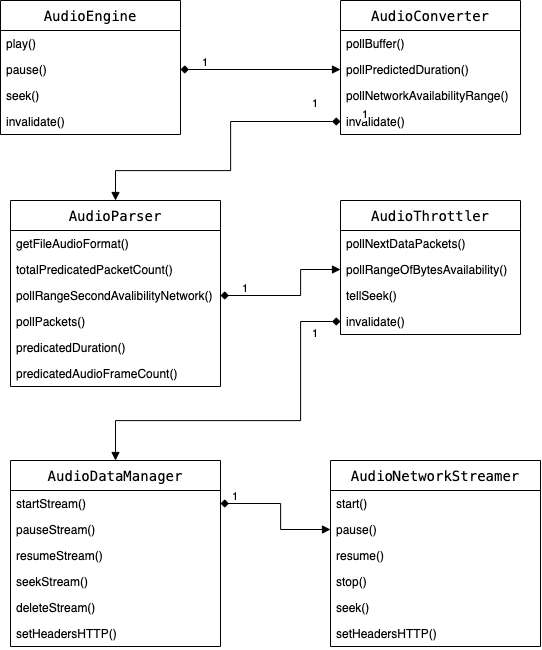
\includegraphics[scale=0.83]{img/class-uml.png}}
            \caption{Диаграмма классов реализуемого программного комплекса.}
            \label{fig:uml}
        \end{figure}

    \subsection{Получение сетевых данных}
        \par Класс AudioDataManager реализует компонент сетевых запросов. 
        С его помощью конфигурируются заголовки HTTP запроса, 
        определяется директория файловой системы устройства для сохранения полученных данных в временных файлах, 
        а также создаётся, прерывается, восстанавливается и очищается поток сетевых данных.
        Интерфейс данного класса представлен в листинге \ref{code:AudioDataManager}.
        \lstinputlisting[label={code:AudioDataManager}, caption={Интерфейс класса AudioDataManager.}]{code/network/AudioDataManager.swift}

        \par Для создания и обработки сетевого запроса применяется композиционный подход: 
        создаётся класс AudioNetworkStreamer, явялющийся частью класса AudioDataManager.
        Класс AudioNetworkStreamer получает сетевые данные, проводит валидацию создаваемого объекта запроса, 
        устанавливает допустимое время обработки запроса, а также проксирует полученные данные классу \newline AudioDataManager.
        Создание и отправка запроса стороне сервера для получения потоковых аудиоданных происходит в методе start.
        
        \par Интерфейс класса AudioNetworkStreamer, а также реализация метода start представлены 
        в листингах \ref{code:AudioNetworkStreamer} и \ref{code:StartFetchData} соответственно.

        \lstinputlisting[label={code:AudioNetworkStreamer}, caption={Интерфейс класса AudioNetworkStreamer.}]{code/network/AudioNetworkStreamer.swift}
        \lstinputlisting[label={code:StartFetchData}, caption={Реализация метода start класса AudioNetworkStreamer.}]{code/network/StartFetchData.swift}


    \subsection{Управление потоком сетевых данных}
        \par Для управления потоком аудиоданных определён класс AudioThrottler.
        Интерфейс класса AudioThrottler предстален в листинге \ref{code:AudioThrottler}. 
        Его интерфейс определяет следующие методы:
        \begin{itemize}
            \item[---] pullNextDataPacket --- отправка буферизированных данных компоненту обработки пакетов;
            \item[---] tellSeek --- определение размера и валидация полученных аудиопакетов;
            \item[---] pollRangeOfBytesAvailable --- вычисление смещения аудиоинформации в битовой форме, находящийся в полученных данных;
            \item[---] invalidate --- очистка буфера приходящих аудиопакетов и прекращение прослушивания сетевой информации;
        \end{itemize}

        \lstinputlisting[label={code:AudioThrottler}, caption={Интерфейс класса AudioThrottler.}]{code/throttler/AudioThrottler.swift}

        \par Логика получения сетевых данных вынесена за пределы публичного интерфейса 
        и определяется при инициализации класса. 
        Создаётся связь между компонентом управления потоком сетевых данных (AudioThrottler) 
        и компонентом получения данных (AudioDataManager) с помощью поведенческого шаблона проектирования <<Издатель-подписчик>>.

        \par Обработчиком данных, полученных из класса AudioThrottler является метод handlerStream. 
        Его реализация представлена в листинге \ref{code:handlerStream}.
        Алгоритм данного метода включает пять пунктов:
        \begin{itemize}
            \item[1.] установка связи (подписка) с классом AudioDataManager для получения сетевых данных;
            \item[2.] определение ожидаемого количества байт сетевой информации, если она пришла;
            \item[3.] проверка размера информации (из первого пункта), а также переполнения буфера приходящих аудиопакетов;
            \item[4.] заполнение буфера новыми сетевыми данными;
            \item[5.] уведомление компонента обработки пакетов о получении новых сетевых данных;
        \end{itemize}

        \lstinputlisting[label={code:handlerStream}, caption={Реализация метода handlerStream.}]{code/throttler/StartStream.swift}
        
    \subsection{Обработка аудиоданных}
        \par Для получения метаинформации и данных аудиосигнала определён класс AudioParser. 
        Его интерфейс представлен в листинге \ref{code:AudioParser}.
        Данный класс получает и обрабатывает информацию о формате аудиофайла, количестве полученных пакетов,
        продолжительности воспроизведения аудиосигнала, пришедшего в сетевых данных, количестве фреймов аудиофайла.

        \par Для вычисления продолжительности воспроизведения аудиосигнала и количества фреймов, 
        находящихся в аудиопакетах, а также для их приведения к системным типам программного интерфейса AudioToolbox 
        определены вычисляемые свойства predictedDuration и totalPredictedAudioFrameCount. 
        Реализации данных методов представлены в листинге \ref{code:ParseData}.

        \lstinputlisting[label={code:AudioParser}, caption={Интерфейс класса AudioParser.}]{code/parser/AudioParser.swift}

        \lstinputlisting[label={code:ParseData}, caption={Реализация методов вычисления продолжительности воспроизведения и количества фреймов.}]{code/parser/ParseData.swift}

        \par Для конвертации и буферизации аудиоданных в PCM буфере определён класс AudioConverter. 
        Процесс буферизации данных происходит в методе класса pullBuffer.
        Реализация метода pullBuffer представлена в листинге \ref{code:PullBuffer}.
        Рассмотрим алгоритм метода:
        \begin{itemize}
            \item[1.] создание PCM буфера, основанное на формате аудиофайла и количестве фреймов;
            \item[2.] определяется количество фреймов для каждого аудиопакета;
            \item[3.] количество пакетов, передающихся в буфер высчитывается как отношение общего количества фреймов к количеству фреймов в одном пакете данных;
            \item[4.] данные приводятся в поток байт;
            \item[5.] проверяется ошибка буферизации;
        \end{itemize}

        \lstinputlisting[label={code:PullBuffer}, caption={Реализация метода pullBuffer.}]{code/converter/PullBuffer.swift}
        
    \subsection{Воспроизведение аудиоданных}
        \par Класс AudioEngine позволяет инициировать воспроизведение аудиоданных. 
        В результате вызова методов данного класса происходит инициализация и настройка AVAudioEngine.
        Для поддержки эффекта ускоренного вопроизведения создаётся список программных аудиоузлов, 
        которые связываются с программным интерфейсом. Данная логика представлена в листинге \ref{code:AudioNodes}.

        \par Корректная обработка аудиоданных со стороны операционной системы осуществляется определением состояния механизма аудиосессии.
        Для его настройки используется класс AVAudioSession, предоставляемый комплексом программных интерфейсов AVFoundation.
        Это позволяет сообщить операционной системе о необходимости воспроизведения аудиосигнала 
        независимо от состояния жизненного цикла программного обеспечения, которое инициировало операцию воспроизведения.

        \lstinputlisting[label={code:AudioNodes}, caption={Cоздание списока программных аудиоузлов.}]{code/audio_engine/AudioNodes.swift}
    \subsection{Пример работы программно-алгоритмического комплекса}
        \par Для демонстрации спроектированного и разработанного программного комплекса был реализован пользовательский интерфейс,
        позволяющий воспроизвести потоковые аудиоданные, 
        предоставляемые серверной частью с использованием прикладного протокола передачи данных HTTP.
        Пользовательский интерфейс представлен на рис. \ref{fig:software-ui}.
        \begin{figure}[!h]
            \center{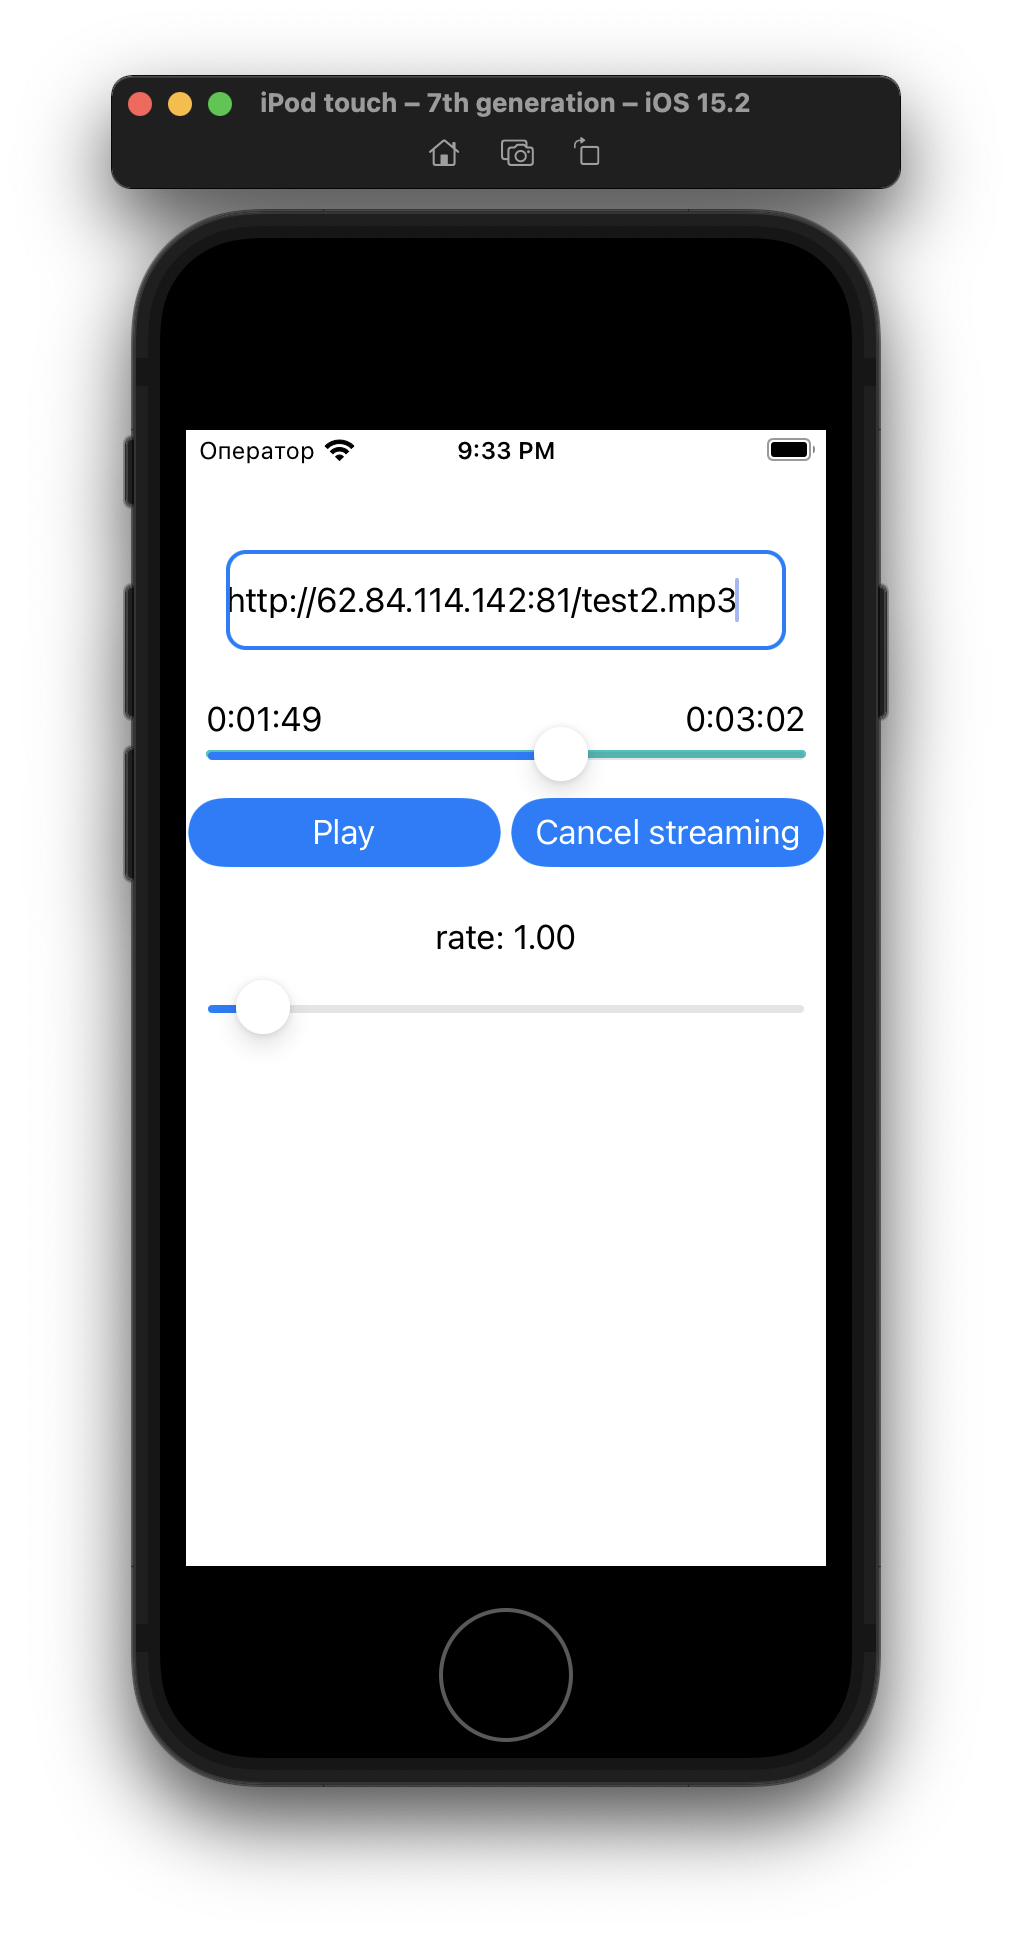
\includegraphics[scale=0.5]{img/ui.png}}
            \caption{Пользовательский интерфейс, для демонстрации функционирования разработанного программного комплекса.}
            \label{fig:software-ui}
        \end{figure}

        \par Для воспроизведения потоковых аудиоданных необходимо в поле ввода передать url адрес, 
        по которому хранится аудиофайл. В процессе получения потока данных становится доступно воспроизведение аудиосигнала
        с возможностью изменения скорости воспроизведения: коэффициент ускорения может принимать значения от $0.1$ до $16$.

        \par Реализованы возможность изменять смещение воспроизведения аудиосигнала (изменять начальное время воспроизведения),
        возможность остановки и восстановления воспроизведения.
        
        \par В процессе получения и обработки сетевых данных происходит логирование процессов и состояний программного комплекса.
        Пример логирования представлен в листинге \ref{code:log}.

        \lstinputlisting[label={code:log}, caption={Логирование процессов и состояний программного комплекса.}]{code/example/logs.txt}
    
    \subsection*{Вывод}
        \par В данном разделе были описаны средства программной реализации, 
        представлены листинги реализации компонентов программного комплекса и отмечены особенности их реализации.
        Приведён пример работы программного комплекса.

\pagebreak